\documentclass{standalone}
\usepackage{../../../../preamble_tikz}
\usepackage{../../../../preamble_math}

\def\r{1}
\def\T{2}
\def\R{4*\r*abs(sin(deg(\T/2)))}
\begin{document}
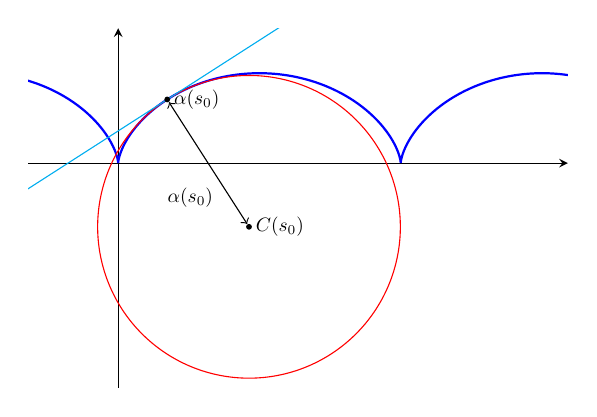
\begin{tikzpicture}[every node/.style={scale=0.7}]
  \begin{axis}[
      axis lines=middle,
      xmin = -2, xmax = 10, %
      ymin = -5, ymax = \r + 2, %
      xtick=\empty, ytick=\empty,
      axis equal image,
    ]
    \addplot[
      domain=-3:10, %Domain of the fucntion
      samples=200, %This parameter determines the number of point to be plotted for the function, while bigger the number better looks the function.
      smooth, %f we use this option, the compiler makes an interpolation between the point plotted to get a soft appearance for the function.
      thick, %Stroke of the function. Options: ultra thin, very thin, thin, semithick, thick, very thick, ultra thick.
      blue, %Color of the function.
    ]({\r*(x-sin(deg(x))},{\r(1-cos(deg(x)))});
    \addplot[
      domain=0:2*pi, %Domain of the fucntion
      samples=200, %This parameter determines the number of point to be plotted for the function, while bigger the number better looks the function.
      smooth, %f we use this option, the compiler makes an interpolation between the point plotted to get a soft appearance for the function.
      thin, %Stroke of the function. Options: ultra thin, very thin, thin, semithick, thick, very thick, ultra thick.
      red, %Color of the function.
    ]({\r*(\T+sin(deg(\T)))+\R*cos(deg(x)},{\r*(-1+cos(deg(\T)))+\R*sin(deg(x)))});
    \addplot[
      domain=-3:2, %Domain of the fucntion
      samples=200, %This parameter determines the number of point to be plotted for the function, while bigger the number better looks the function.
      smooth, %f we use this option, the compiler makes an interpolation between the point plotted to get a soft appearance for the function.
      thin, %Stroke of the function. Options: ultra thin, very thin, thin, semithick, thick, very thick, ultra thick.
      cyan, %Color of the function.
    ]({\r*(\T-sin(deg(\T))+\r*x*(1-cos(deg(\T))},{\r(1-cos(deg(\T)))+\r*x*sin(deg(\T))});
    \node[circle,fill=black,inner sep=0pt,minimum height=3pt](a) at ({\r*(\T-sin(deg(\T))},{\r(1-cos(deg(\T)))}){};
    \node[circle,fill=black,inner sep=0pt,minimum height=3pt](b) at ({\r*(\T+sin(deg(\T)))},{\r*(-1+cos(deg(\T)))}){};
    \node[anchor=west] at (a){$\vf{\alpha}(s_0)$};
    \node[anchor=west] at (b){$C(s_0)$};
    \draw[<->] (a) -- (b) node[pos=0.65,anchor=north east]{$\rh\alpha(s_0)$};
  \end{axis}
\end{tikzpicture}
\end{document}